\section{Profiling performance and power consumption}

For the perception algorithm, the first stage of our method is profiling the performance (timing and, if available, quality) and power consumption of the computation. 
To do this profiling, we first navigate the robot manually in corridors and log video from the on-board camera at a high frame-rate. 
We run Vanishing point on this video offline and profile it with different scheduling of the three components (Blur, Canny and Hough) on the CPU and GPU, and at different frequencies of both processors (Fig. \ref{fig:vanishing}).

We wrote a custom C-code library to log power measurements from a Tektronix PWS4205 Programmable DC power supply at 100Hz. 
For this we communicate with the power supply over USB using the USB Test and Measurement Class (USB-TMC) communication protocol. 

%In order to profile the timing performance of the Vanishing point algorithm with different schedules for the three tasks we allocate on either the CPU or the GPU, and the different clock frequencies for the CPU and the GPU, we have a script that runs the vanishing point algorithm for all settings offline and logs the update rate in Hz as well as individual execution times of the components and the power consumption. 
Since for an algorithm like Vanishing point there is no well-defined notion of ground truth, we do not have a measure of accuracy of the algorithm. 
Instead, Vanishing point's update rate is used as a performance measure, since with faster updates the controller can apply input signals to the car faster, resulting in better control performance. 


\subsection{Results}

Figures \ref{fig:dfsa}, \ref{fig:sfda} show the profiling results for the update rate of the Vanishing Point algorithm for different CPU-GPU allocations of the 3 tasks and different frequencies of the CPU and the GPU. Note, the CPU can be clocked upto 2.32 GHz (on all 4 cores), while the GPU can be clocked upto 0.852 GHz. We select 6 operating frequencies evenly spaced from the minimum and maximum Jetson CPU and GPU frequencies for both the CPU and the GPU. Also note that in these figures, Note, the 3 alphabet combinations imply the resource allocated to the Blur, Canny and Hough transform tasks respectively, e.g. C G C means that the Blur was on the CPU, Canny on the GPU and the Hough transform no the CPU and so on.


\begin{figure}[hbtp]
\centering
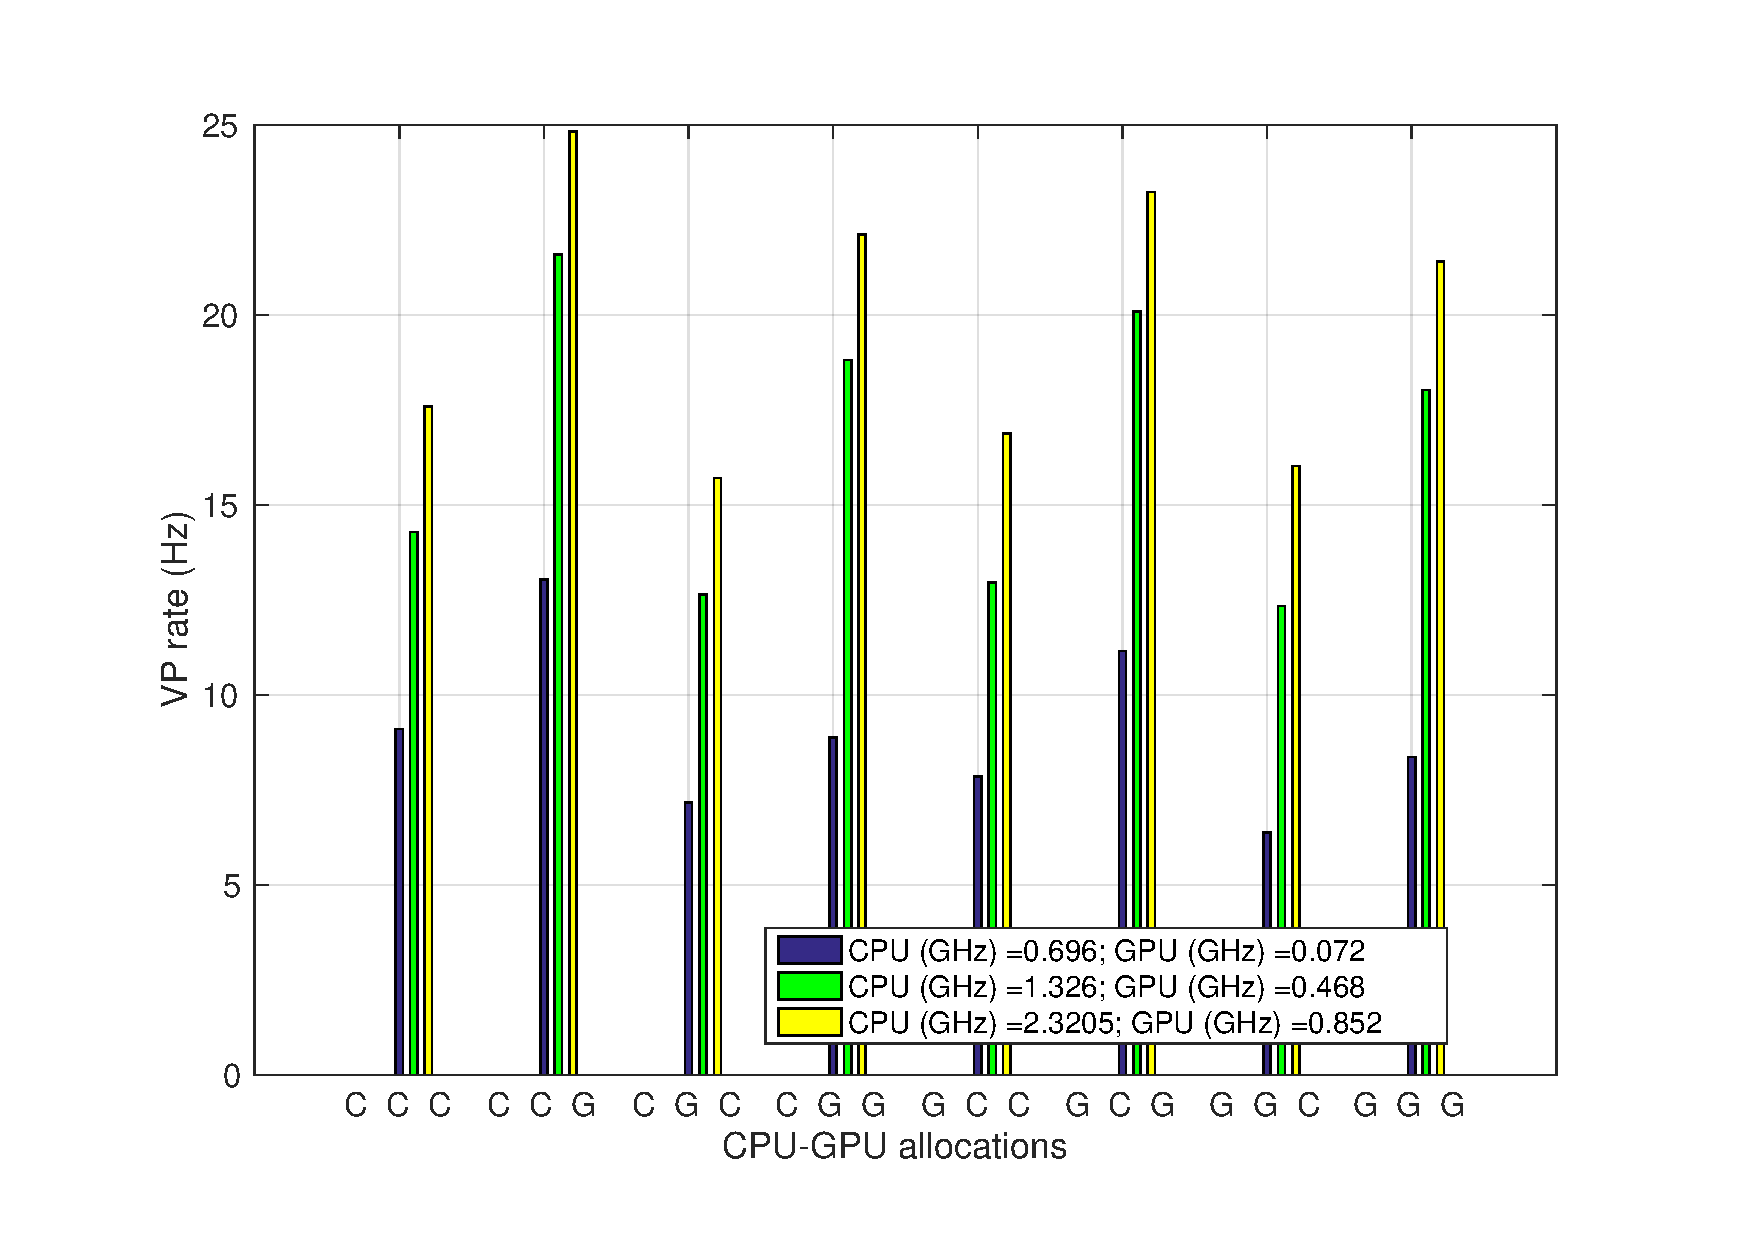
\includegraphics[width=0.46\textwidth]{Data/figs/RateHist.pdf}
\caption{Update rate for different frequencies and a given CPU-GPU assignment. For brevity we only consider 3 CPU and GPU frequencies for this figure, ranging from the minimum and maximum of both the CPU and the GPU. }
\label{fig:dfsa} %diff freq same assignment}
\end{figure}

\begin{figure}[htbp]
	\centering
	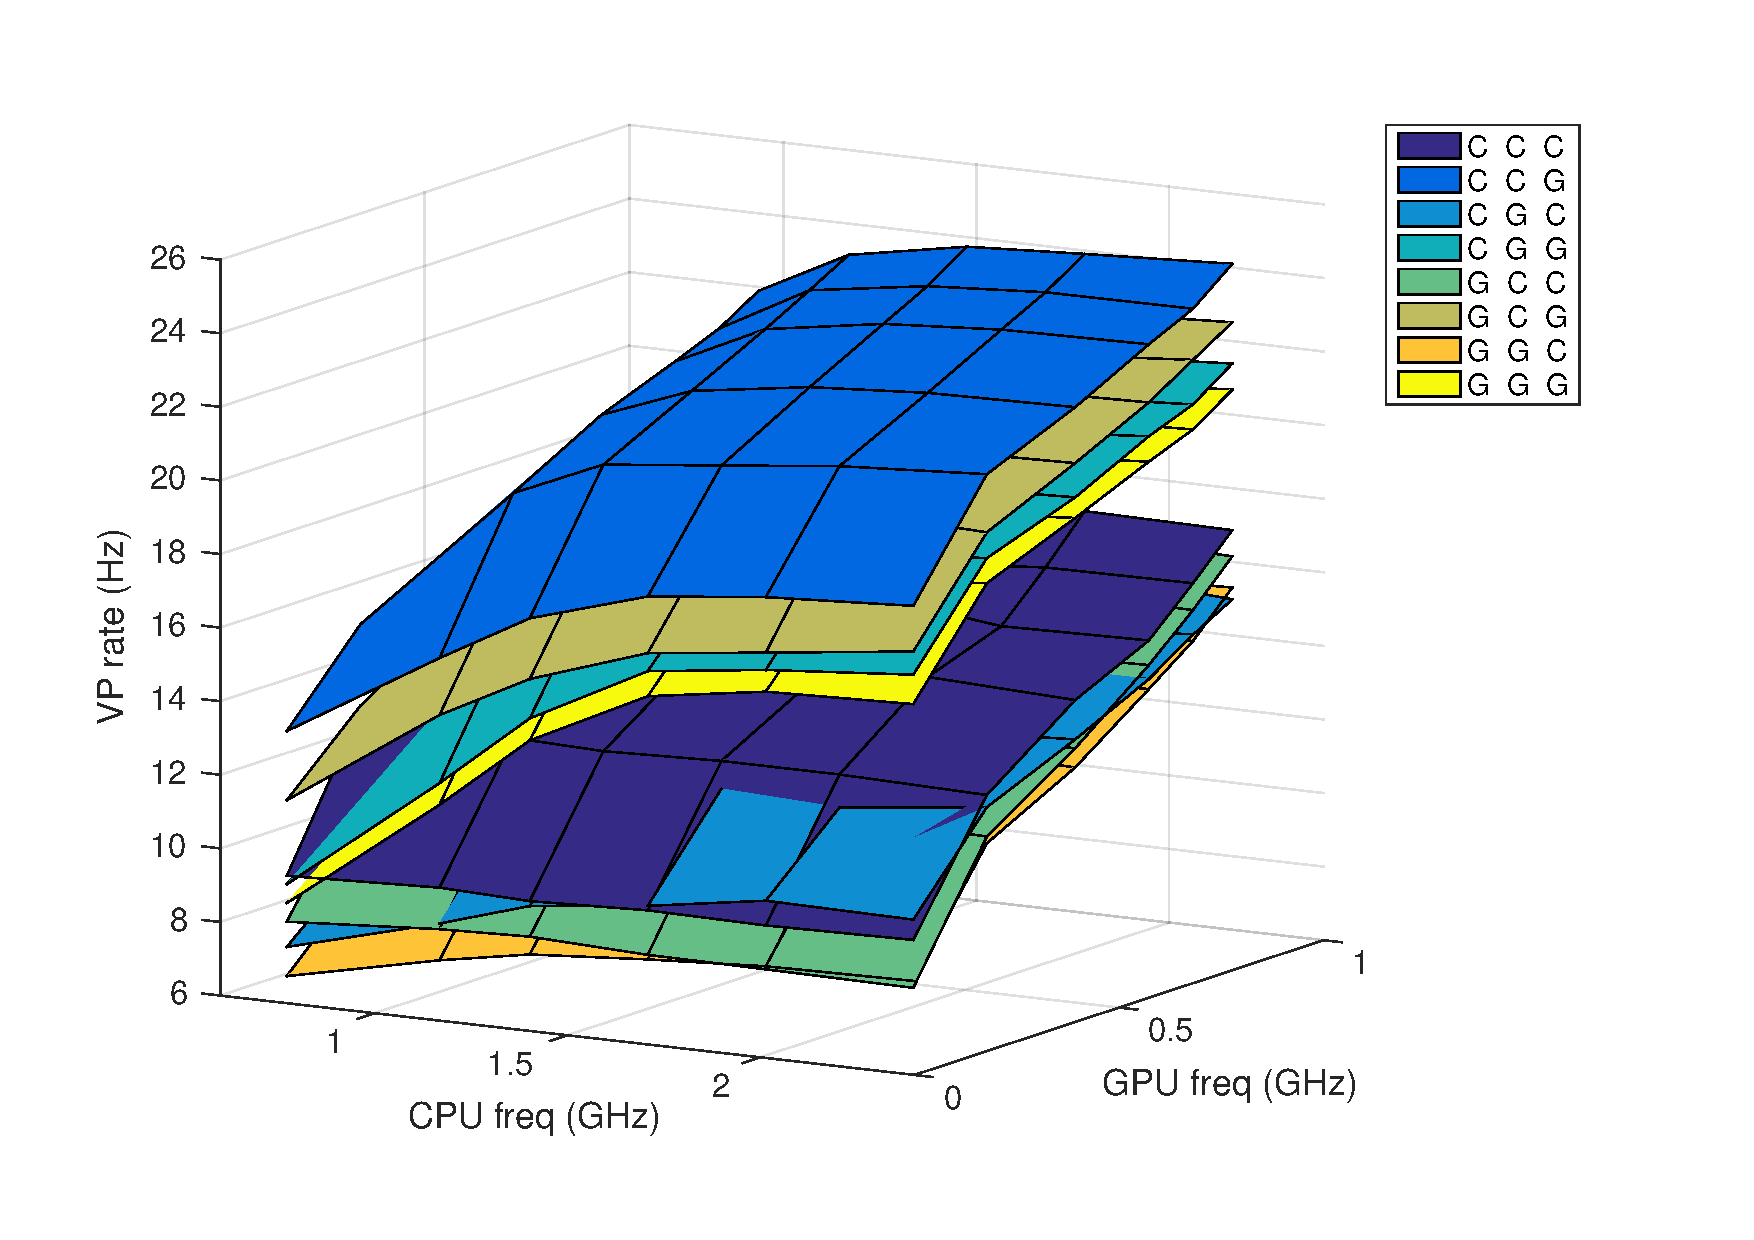
\includegraphics[width=0.46\textwidth]{Data/figs/surf_Rate.pdf}
	\caption{Update rate for different CPU-GPU assignments at fixed frequencies.}
	\label{fig:sfda}%same freq diff assignment}
\end{figure}

Figures \ref{fig:dfsa_pow}, \ref{fig:sfda_pow} show the profiling of average power consumed during the computations for the vanishing point over all frames in the video used for the profiling.


\begin{figure}[htbp]
\centering
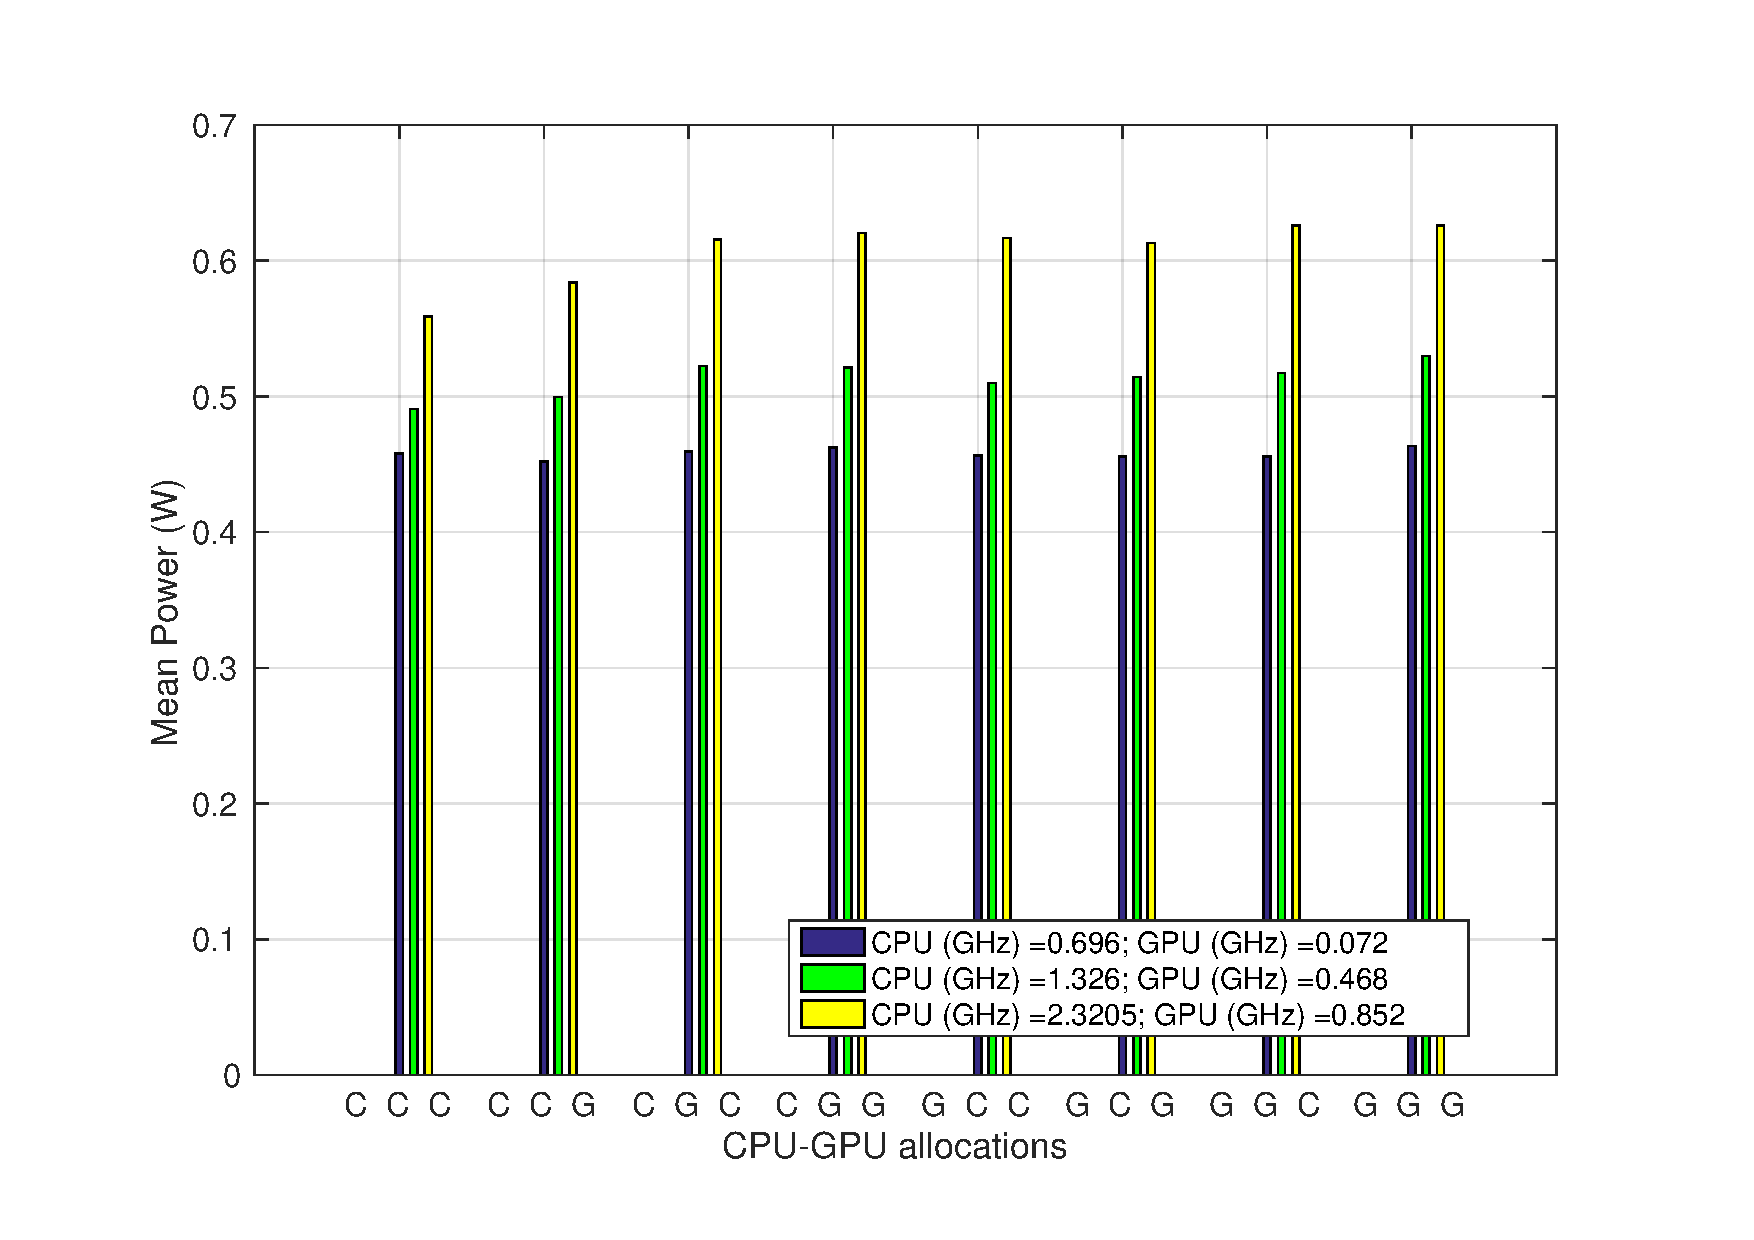
\includegraphics[width=0.46\textwidth]{Data/figs/PowerHist.pdf}
\caption{Mean Power consumed by the Jetson for different frequencies and a given CPU-GPU assignment.  For brevity we only consider 3 CPU and GPU frequencies for this figure, ranging from the minimum and maximum of both the CPU and the GPU.}
\label{fig:dfsa_pow} %diff freq same assignment}
\end{figure}

\begin{figure}[htbp]
	\centering
	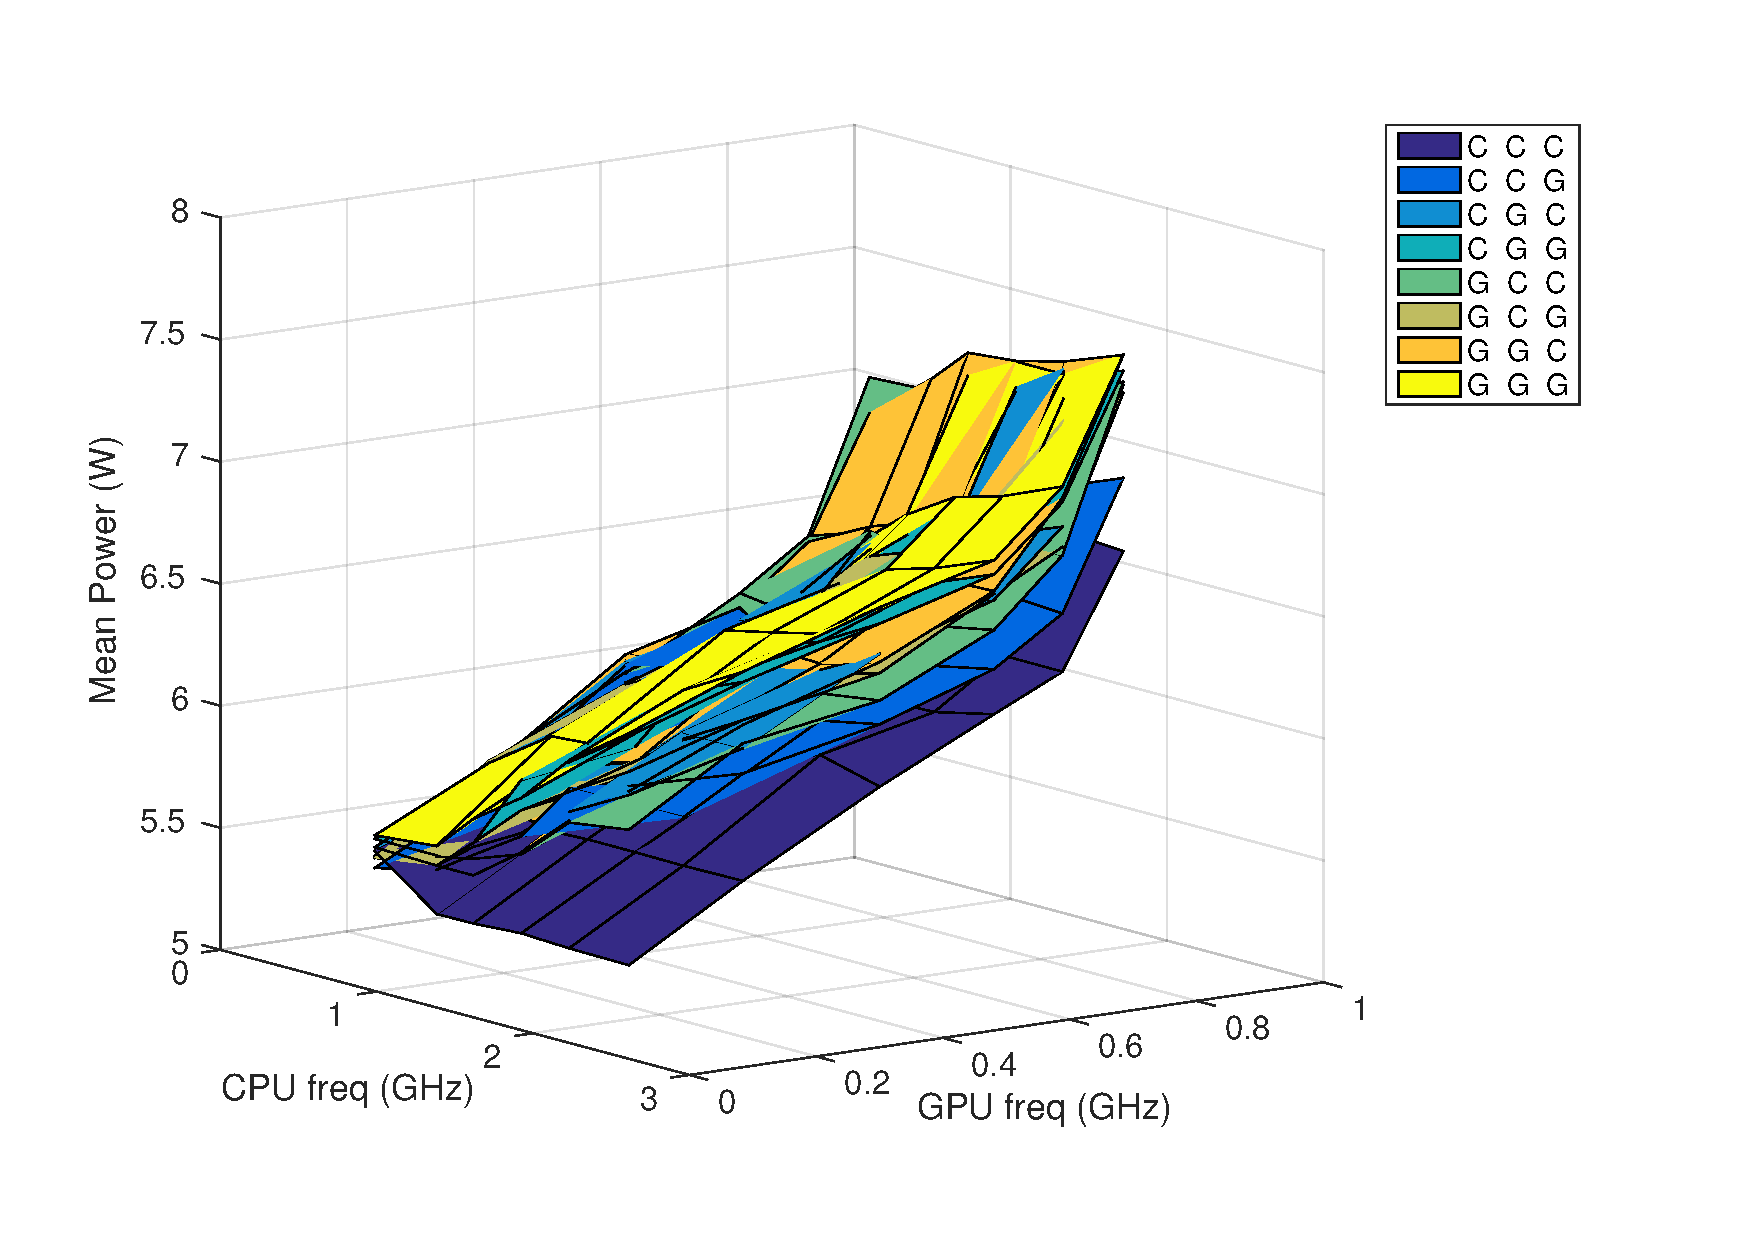
\includegraphics[width=0.46\textwidth]{Data/figs/surf_Power.pdf}
	\caption{Mean Power consumed by the Jetson for different CPU-GPU assignments at fixed frequencies.}
	\label{fig:sfda_pow}%same freq diff assignment}
\end{figure}



